%----------------------------------------------------------------------------------------
%	PACKAGES AND THEMES
%----------------------------------------------------------------------------------------
\documentclass{beamer}
% Load a bunch of useful packages:
\usepackage{amssymb,amsmath,amsfonts,mathtools} % useful math fonts and symbols
\usepackage{geometry} % allows changing margins and sizes of stuff
\usepackage{hyperref} % allows referencing of lines of text, urls, figures etc
\usepackage{natbib} % allows citation referencing from a .bib file
\bibliographystyle{apalike} % American Psychological Association style guide
\usepackage{graphicx} % to include graphics from the figures folder with helpful formating options
\usepackage{tikz}
\usetikzlibrary{arrows}
\usepackage{pgfplots}
\usetikzlibrary{calc}
%---------------------------------------------%
\usepackage{color} % custom color definitions:%
    %UOregon colors:                          %
    \definecolor{UOGreen}{RGB}{18, 71, 52}    %
    \definecolor{UOYellow}{RGB}{254, 225, 35} %
    %Secondary official colors:               %
    \definecolor{LegacyGreen}{HTML}{104735}   %
    \definecolor{GrassGreen}{HTML}{489D46}    %
    \definecolor{LimeGreen}{HTML}{8ABB40}     %
    \definecolor{Chartreuse}{HTML}{E2E11B}    %
    \definecolor{Berry}{HTML}{8D1D58}         %
    \definecolor{DarkBlue}{HTML}{004F6E}      %
    \definecolor{LightBlue}{HTML}{00A5B5}     %
    \definecolor{crimson}{RGB}{ 170, 4, 36 }
    \definecolor{darkblue}{RGB}{ 4, 47, 170 }
    \definecolor{brown}{RGB}{ 111, 71, 2 }
    \definecolor{periwinkle}{RGB}{ 90, 177, 204 }
    \definecolor{ducksgreen}{HTML}{007030}
%----------------------------------------------

\usepackage{setspace} % to specify single, double or one-half spacing of text
\usepackage{indentfirst} % indent first line of a text paragraph
\usepackage{multicol} %multipage ability
\usepackage{multirow}
\usepackage{ulem} % \ul (underline) command which will break over line ends
\usepackage{amsthm} % allows standarized theorem commands
\setbeamertemplate{theorems}[numbered]
\theoremstyle{plain}
\newtheorem{assume}{Assumption}
\newtheorem{define}{Definition}
\usepackage{breqn} %automatic line breaking
\normalem

% Theming and Appearance Setup:
\usetheme{metropolis}
\metroset{block=fill}
%\usetheme{default}
\usefonttheme{professionalfonts}
\fontfamily{ppl}\selectfont
\usecolortheme[named=UOGreen]{structure}
\setbeamertemplate{footline}[frame number]
\setbeamertemplate{headline}{} %Removes Section Index on top of slide
\beamertemplatenavigationsymbolsempty
\hypersetup{
    colorlinks=true,
    linkcolor=DarkBlue,
    filecolor=Berry,
    citecolor=GrassGreen,
    urlcolor={LightBlue},
    pdftitle={Trade and Labor Market Dynamics},
    pdfpagemode=FullScreen
}

%------------------------------------------------------------------------------%TITLE PAGE
%------------------------------------------------------------------------------
% The title
\title{Strategic Moves}
\author{Dante Yasui }
\institute{EC327 Game Theory}
\date{Winter 2024}
\titlegraphic{
\includegraphics[scale=.4]{UOSignature-356.png}}


%-----------------------------------------------------------------------------
%	PRESENTATION SLIDES
%-----------------------------------------------------------------------------

\begin{document}

\begin{frame}[plain]
    % Print the title page as the first slide
    \titlepage
\end{frame}
\addtocounter{framenumber}{-1}

\begin{frame}[plain]{Outline}
  \tableofcontents
\end{frame}
\addtocounter{framenumber}{-1}

% - - - - - - - - - - - - - - - - - - - - - - - - - - - - - - - - - - - - - -

\begin{frame}{}
  \begin{itemize}
    \item So far, we have taken the \textbf{rules of a game} as fixed. 
    \item But in many cases, the very structure of a game can be 
    \alert{strategically manipulated} by certain players.
  \end{itemize}
\end{frame}

% - - - - - - - - - - - - - - - - - - - - - - - - - - - - - - - - - - - - - - -

\begin{frame}{}
  \begin{itemize}
    \item We have already talked about how different types of games 
    favor some agents over others 
    \begin{itemize}
      \item I.e., first mover advantage, 
      \item second mover advantage, 
      \item asymmetric info 
    \end{itemize}
    \item So it would make sense that if players can \textit{manipulate}
    the rules of a game in their favor, they will try to do so.
  \end{itemize}  
\end{frame}

% - - - - - - - - - - - - - - - - - - - - - - - - - - - - - - - - - - - - - -

\begin{frame}{}
  \begin{itemize}
    \item We can think about adding a first-stage to our original game 
    \begin{itemize}
      \item \textbf{First Stage:} specify how you will act in second stage 
      \item \textbf{Second Stage:} the original game
      \begin{itemize}
        \item but now players set their beliefs based on what happened
        in the first stage.
      \end{itemize}
    \end{itemize}
  \end{itemize}  
\end{frame}

% - - - - - - - - - - - - - - - - - - - - - - - - - - - - - - - - - - - - - -

\begin{frame}{}
  \begin{itemize}
    \item Different first stage actions correspond to what we will call:
    \begin{itemize}
      \item \alert{commitments},
      \item \alert{threats},
      \item or \alert{promises}
    \end{itemize}
    \item Whether any of these actions is \textbf{effective}
    depends on the beliefs of the other player(s).
    \begin{itemize}
      \item The \alert{credibility} of a strategic move \textit{matters}.
    \end{itemize}
  \end{itemize} 
\end{frame}

% - - - - - - - - - - - - - - - - - - - - - - - - - - - - - - - - - - - - - -

\begin{frame}{}
  Examples of Strategic Moves:
  \begin{itemize}
    \item Amazon publicly \textit{commits} to going carbon neutral by 2040
    \item Parents \textit{promise} "you will get a PS5 if you get all A's" 
    to their children
    \item Nuclear powers \textit{threaten} "Mutually Assured Destruction"
    to each other in \alert{brinksmanship} games
  \end{itemize}
\end{frame}

% - - - - - - - - - - - - - - - - - - - - - - - - - - - - - - - - - - - - - - -

\begin{frame}{}
  Conditional Strategic Moves 
  \begin{itemize}
    \item I might declare a \textbf{response rule} 
    which is a move that depends on someone else's behavior
    \item I might try to take action to stop someone from doing something 
    through a \textbf{deterrence} strategy
    \item Or I could try to get someone to do something 
    through \textbf{compellence}
    \item \textbf{deterrence} or \textbf{compellence} could take the form 
    of a \alert{threat} or \alert{promise}:
    \begin{itemize}
      \item A \alert{threat}: 
      "Unless your action conforms to what I want, then I will \textit{harm} you"
      \item A \alert{promise}:
      "If your action conforms to what I want, I will \alert{reward} you"
    \end{itemize}
  \end{itemize}
\end{frame}

% - - - - - - - - - - - - - - - - - - - - - - - - - - - - - - - - - - - - - - -

\begin{frame}{What does it mean to move first?}
  \begin{itemize}
    \item An action must be both \textbf{observable} and \textbf{irreversible}.
    \item If an action is \textit{unobservable}, 
    then other players can't react to it.
    \item If an action is \textit{reversible},
    then the `first-mover' could change their action in reaction to another move.
  \end{itemize} 
\end{frame}

\section{Classification of Strategic Moves}
% Section 1: A Classification of Strategic Moves
%-------------------------------------------------------------------------------

\begin{frame}{Unconditional Strategic Moves}
  \textbf{\alert{Commitment}}
  \begin{itemize}
    \item If a player makes an observable and irreversible move to 
    \textbf{limit} their future actions.
    \item ``In the game to follow, I will make a particular move, $X$''
  \end{itemize} 
\end{frame}

% - - - - - - - - - - - - - - - - - - - - - - - - - - - - - - - - - - - - - - - 

\begin{frame}{Unconditional Strategic Moves}
  When does \textbf{\alert{Commitment}} matter?
  \begin{itemize}
    \item When it changes the beliefs of other players
    \item This can rely on the \alert{credibility} of certain commitments.
  \end{itemize} 
\end{frame}

% - - - - - - - - - - - - - - - - - - - - - - - - - - - - - - - - - - - - - - - 

\begin{frame}{Unconditional Strategic Moves}
  \begin{center}
    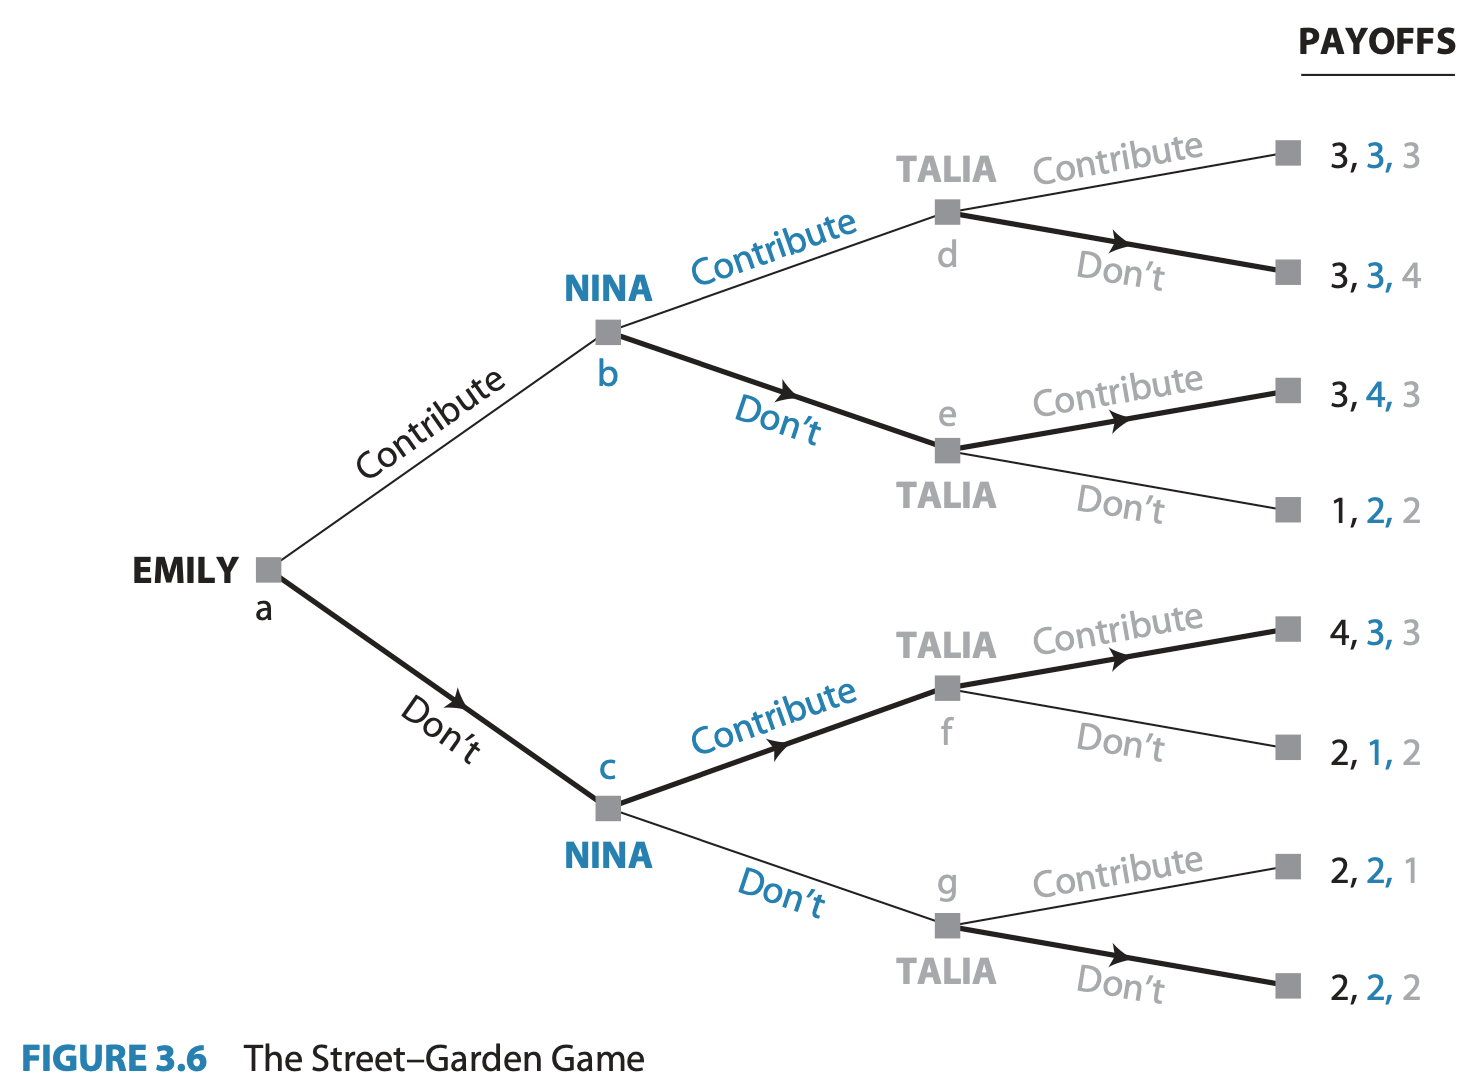
\includegraphics[width=.6\textwidth]{figures/fig3.6.png}
  \end{center}
  Recall that the Street-Garden Game ended with \alert{Emily} \textit{not contributing},
  knowing that both \alert{Nina} and \alert{Talia} \textit{would contribute}.
\end{frame}

% - - - - - - - - - - - - - - - - - - - - - - - - - - - - - - - - - - - - - - - 

\begin{frame}{Unconditional Strategic Moves}
  \begin{center}
    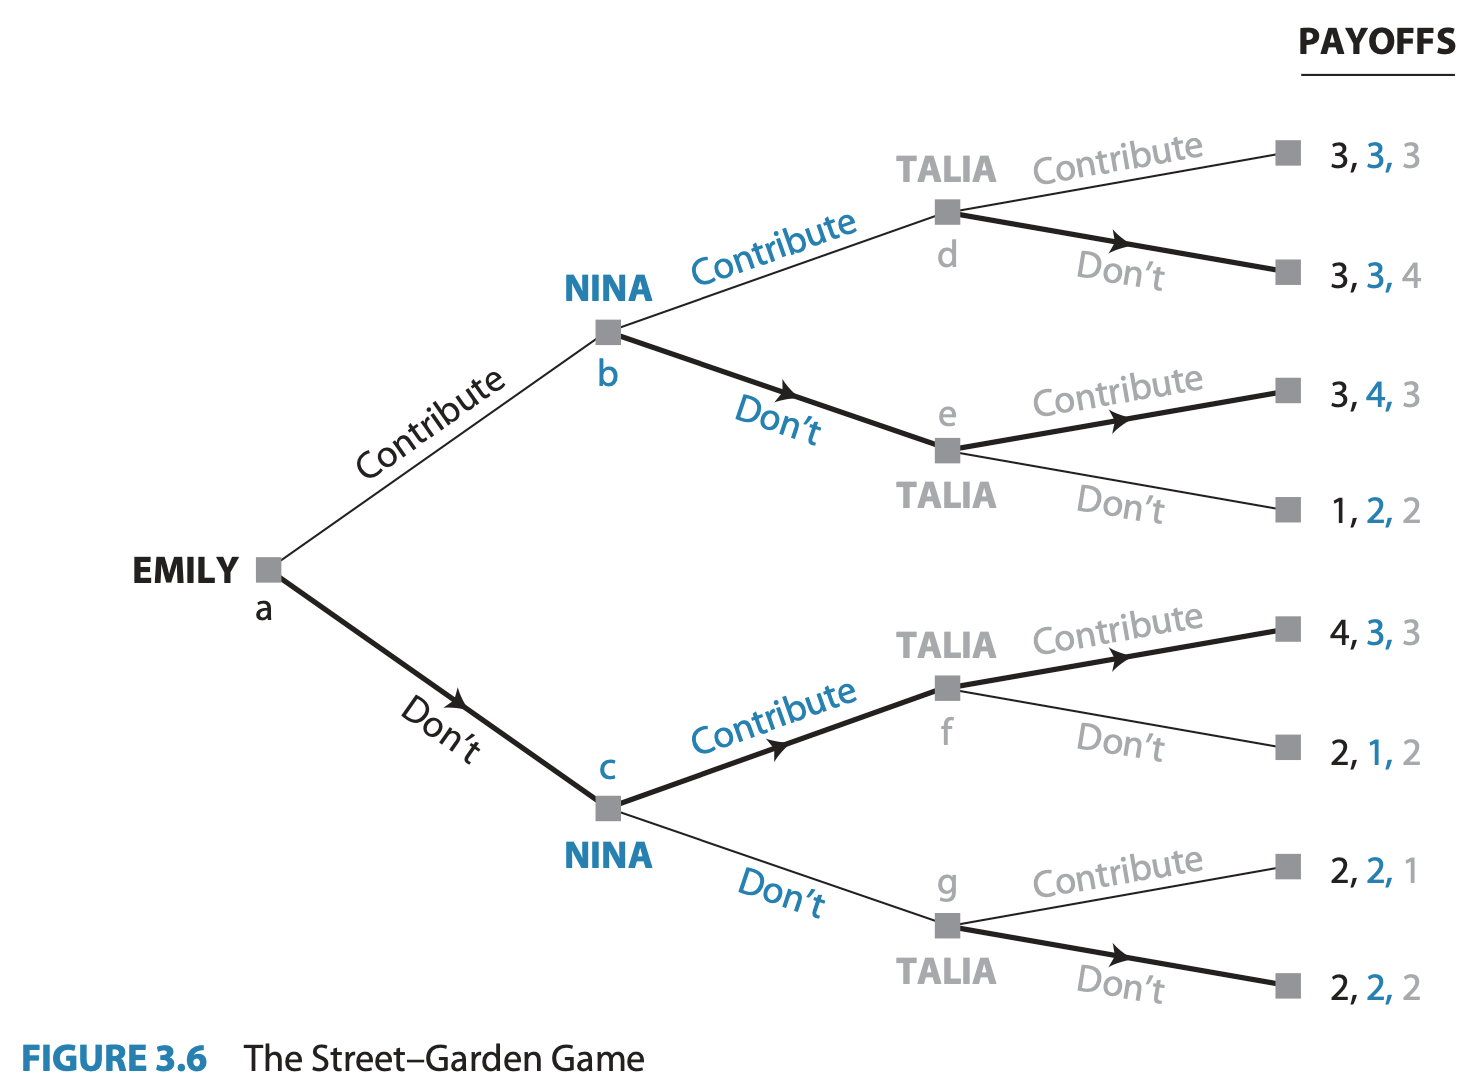
\includegraphics[width=.6\textwidth]{figures/fig3.6.png}
  \end{center}
  But what if either \alert{Nina} or \alert{Talia} can 
  \textbf{commit} to \textit{not contributing}? \\ 
  Maybe \alert{Talia} could let everyone know that she has sunk all of her savings into an expensive home renovation.
\end{frame}

% - - - - - - - - - - - - - - - - - - - - - - - - - - - - - - - - - - - - - - - 

\begin{frame}{Conditional Strategic Moves}
  \textbf{\alert{Response Rules}} 
  \begin{itemize}
    \item If a player makes an observable and irreversible plan that is \textbf{conditional} on another player's actions. 
    \item ``In the game to follow, I will respond to your choices in the following way.
    If you choose $Y_1$, I will do $Z_1$, if you do $Y_2$, I will do $Z_2$, ...''
  \end{itemize}
\end{frame}

% - - - - - - - - - - - - - - - - - - - - - - - - - - - - - - - - - - - - - - - 

\begin{frame}{Conditional Strategic Moves}
  Types of conditional strategic moves
  \begin{itemize}
    \item \alert{Deterrence}: when the first player wants to \textit{stop} another player from making some action
    \item \alert{Compellence}: when the first player wants to \textit{induce} another player to do something 
  \end{itemize}
\end{frame}

% - - - - - - - - - - - - - - - - - - - - - - - - - - - - - - - - - - - - - - - 

\begin{frame}{Conditional Strategic Moves}
  Methods of achieving \textit{deterrence} or \textit{compellence} 
  \begin{itemize}
    \item \alert{Threat}: \\
    ``Unless you do as I want, I will act to make you worse off''
    \item \alert{Promise}: \\
    ``If you do as I want, I will act to make you better off''
  \end{itemize}
\end{frame}

% - - - - - - - - - - - - - - - - - - - - - - - - - - - - - - - - - - - - - - - 

\begin{frame}{Credibility}
  What distinguishes an effective strategic move from \textbf{cheap talk}?
  \begin{itemize}
    \item Any player can promise or threaten anything they like, 
    but whether it works to change other people's behavior depends on its \alert{credibility}
    \item An effective \textit{threat} will be \textbf{costly} to the person doing the threatening.
  \end{itemize}
\end{frame}

% - - - - - - - - - - - - - - - - - - - - - - - - - - - - - - - - - - - - - - - 

\begin{frame}{Split or Steal - Revisited}
  Recall the clip from \href{https://youtu.be/S0qjK3TWZE8}{Golden Balls} we watched with Nick and Ibrahim 
  \begin{itemize}
    \item How would you characterize Nick's strategic move here? 
    \item \alert{Unconditional} or \alert{Conditional}?
    \item \alert{deterrence} or \alert{compellence}?
    \item What parts of Nick's story are \alert{credible}?
  \end{itemize}
\end{frame}


\section{Commitments}
% Section 2: Commitments
%------------------------------------------------------------------------------

\begin{frame}{Game of Chicken}
  \begin{table}[!h]
		\centering
		\begin{tabular}{cr|c|c|}
			& \multicolumn{1}{c}{} & \multicolumn{2}{c}{Dean}\\
			& \multicolumn{1}{c}{} & \multicolumn{1}{c}{Swerve} & \multicolumn{1}{c}{Straight} \\\cline{3-4}
			\multirow{2}*{James} & Swerve & 0,0 & -1,1 \\\cline{3-4}
			& Straight & 1,-1 & -2, -2 \\\cline{3-4}
		\end{tabular}
	\end{table}
  \begin{itemize}
    \item How many Nash Equilibria are there? 
    \item Which of the equilibria would \textbf{James} prefer?
  \end{itemize}
\end{frame}

% - - - - - - - - - - - - - - - - - - - - - - - - - - - - - - - - - - - - - - - 

\begin{frame}{Game of Chicken with Commitment}
  \begin{center}
    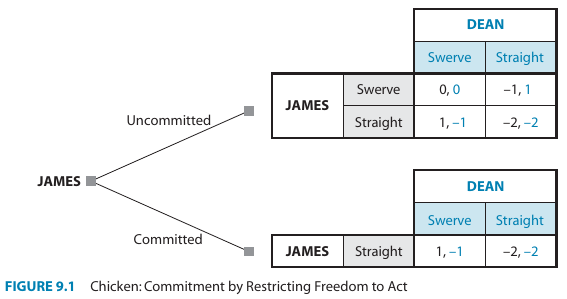
\includegraphics[width=.9\textwidth]{figures/fig91.png} 
  \end{center} 
  What would the outcome of this game be?
\end{frame}

% - - - - - - - - - - - - - - - - - - - - - - - - - - - - - - - - - - - - - - - 

\begin{frame}{Game of Chicken with Commitment}
  \begin{center}
    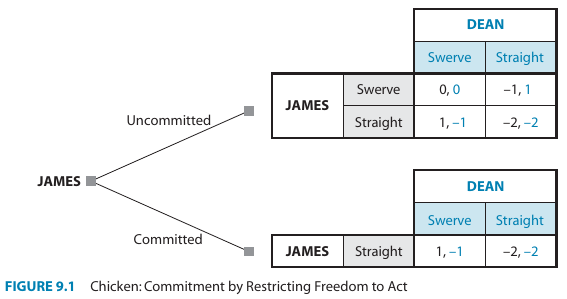
\includegraphics[width=.6\textwidth]{figures/fig91.png} 
  \end{center} 
  How can James make this commitment \textit{credible}?
  \begin{itemize}
    \item Irreversible 
    \item Visible to Dean
  \end{itemize}
\end{frame}

% - - - - - - - - - - - - - - - - - - - - - - - - - - - - - - - - - - - - - - - 

\begin{frame}{Game of Chicken with Commitment}
  \begin{center}
    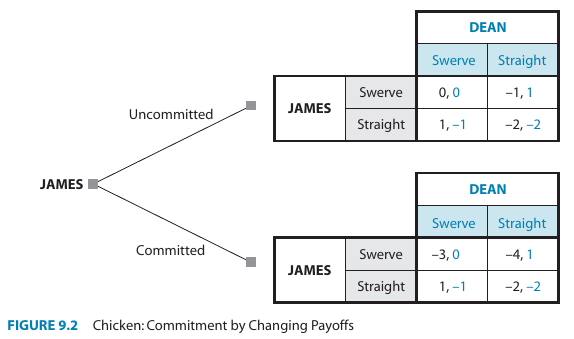
\includegraphics[width=.8\textwidth]{figures/fig92.png} 
  \end{center} 
  James could also change his payoffs; maybe by gaining a \textit{reputation} 
  in repeated play of chicken so he would be humiliated if he ever swerves
\end{frame}

\begin{frame}{Optimal Commitment in Larger Games}
  \begin{table}[!h]
		\centering
		\begin{tabular}{cr|c|c|c|}
			& \multicolumn{1}{c}{} & \multicolumn{3}{c}{$P_2$}\\
      & \multicolumn{1}{c}{} & \multicolumn{1}{c}{X} & \multicolumn{1}{c}{Y} & \multicolumn{1}{c}{Z} \\\cline{3-5}
      \multirow{3}*{$P_1$} & A & 4,4 & 1,5 & 0,0 \\\cline{3-5}
      & B & 3,1 & 2, 2 & 5,1 \\\cline{3-5}
      & C & 1,1 & 1,3 & 4,4 \\\cline{3-5}
		\end{tabular}
	\end{table}
  What is the (pure strategy) Nash Equilibrium? \\
  Which strategy should $P_1$ commit to? 
\end{frame}


\section{Threats and Promises}
% Section 3: Threats and Promises
%-------------------------------------------------------------------------------

\begin{frame}{Examples of Threats and Promises}
  \begin{center}
    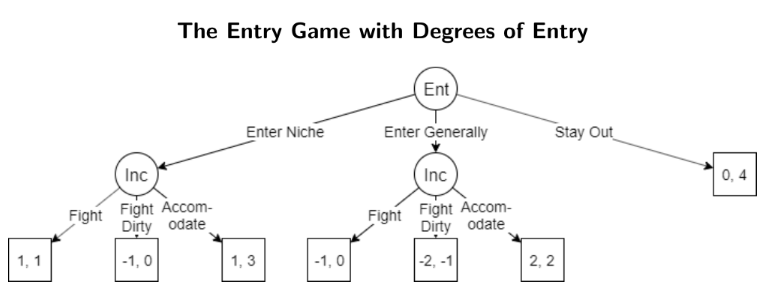
\includegraphics[width=1\textwidth]{figures/entrygame.png} 
  \end{center} 
  What is the \textbf{SPNE}?
\end{frame}

% - - - - - - - - - - - - - - - - - - - - - - - - - - - - - - - - - - - - - - - 

\begin{frame}{Examples of Threats and Promises}
  \begin{center}
    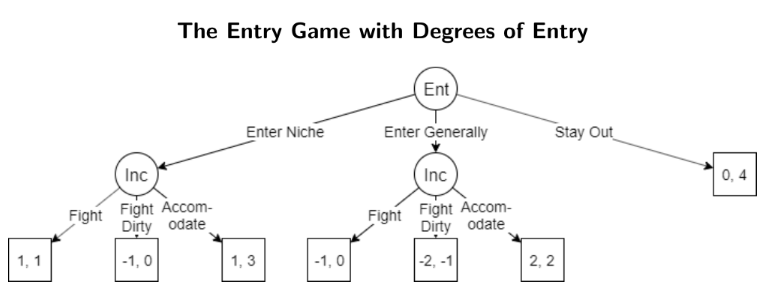
\includegraphics[width=.7\textwidth] {figures/entrygame.png}
  \end{center} 
  Examples of threats/promises that \alert{Incumbent} could make:
  \begin{itemize}
    \item ``If you enter niche, I will Fight; If you enter generally, I will Fight Dirty''
    \item ``If you enter niche, I will Accommodate; If you enter generally, I will Fight''
    \item ``If you enter niche \textit{or} generally, I will Fight Dirty''
  \end{itemize}
\end{frame}

% - - - - - - - - - - - - - - - - - - - - - - - - - - - - - - - - - - - - - - - 

\begin{frame}{Examples of Threats and Promises}
  \begin{center}
    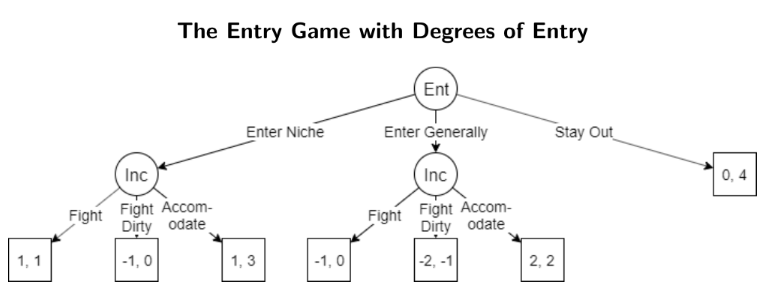
\includegraphics[width=.7\textwidth] {figures/entrygame.png}
  \end{center} 
  What is the \textbf{optimal commitment} for the \alert{Incumbent} to make? \\
  How can they be made credible?
\end{frame}

% - - - - - - - - - - - - - - - - - - - - - - - - - - - - - - - - - - - - - - - 

\begin{frame}{Examples of Threats and Promises}
  \begin{center}
    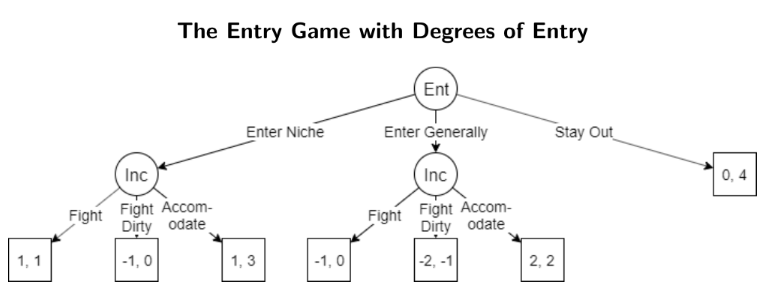
\includegraphics[width=.7\textwidth] {figures/entrygame.png}
  \end{center} 
  {Stay Out, (Fight Dirty, Fight)} \textit{is} a NE of this game, just not \textit{subgame-perfect}
  \begin{itemize}
    \item An interpretation for those non-subgame-perfect NEs is that they exist as the result of such threats 
  \end{itemize}
\end{frame}

% - - - - - - - - - - - - - - - - - - - - - - - - - - - - - - - - - - - - - - - 

\begin{frame}{Examples of Threats and Promises}
  \begin{center}
    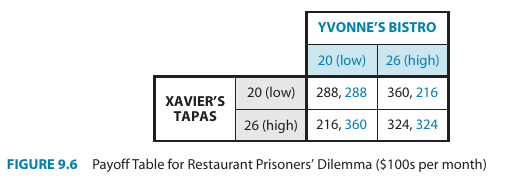
\includegraphics[width=.8\textwidth]{figures/fig96.png} 
  \end{center} 
  Consider the promise ``I will charge a high price if you do'' \\
  Sounds good right?
\end{frame}

% - - - - - - - - - - - - - - - - - - - - - - - - - - - - - - - - - - - - - - - 

\begin{frame}{Examples of Threats and Promises}
  \begin{center}
    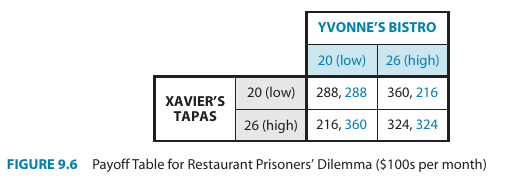
\includegraphics[width=.6\textwidth]{figures/fig96.png} 
  \end{center}
  What if Xavier \textit{promises} to set a high price?
  \begin{itemize}
    \item Should Yvonne believe him? 
    \item How can Xavier \textit{credibly commit} to not undercutting Yvonne when he sees she has set a high price?
    \begin{itemize}
      \item Handing off the decision to a trusted 3rd party (commitment),
      \item Develop a reputation of honesty (change his payoffs)
    \end{itemize}
  \end{itemize}
\end{frame}

% - - - - - - - - - - - - - - - - - - - - - - - - - - - - - - - - - - - - - - - 

\begin{frame}{Deterrence of Entry (Harrington)}
  \begin{center}
    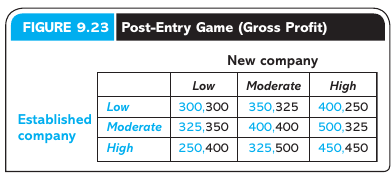
\includegraphics[width=.6\textwidth]{figures/fig923.png} 
  \end{center}
  Consider a market with an established and a potential new entrant:
  \vspace{-5mm}
  \begin{itemize}
    \item Established monopolist would usually earn 1,000 profit 
    \item If competing, each company could set \textit{low}, \textit{moderate}, \textit{high} price
    \item Start-up cost to entrant is 350.
  \end{itemize}
\end{frame}

% - - - - - - - - - - - - - - - - - - - - - - - - - - - - - - - - - - - - - - - 

\begin{frame}{Deterrence of Entry}
  \begin{center}
    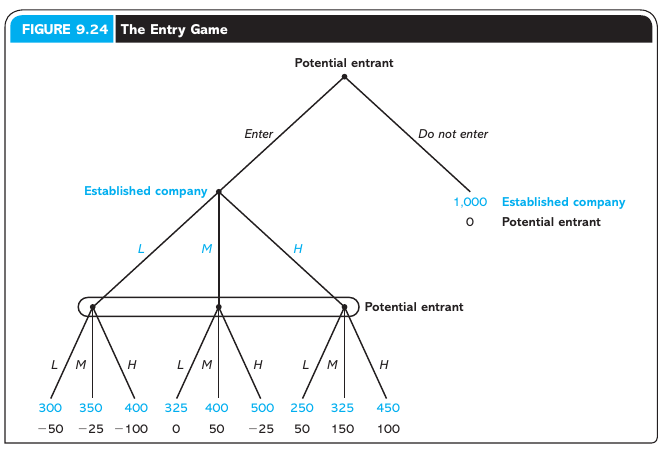
\includegraphics[width=.9\textwidth]{figures/fig924.png}
  \end{center} 
  What is the \textbf{SPNE}?
\end{frame}

% - - - - - - - - - - - - - - - - - - - - - - - - - - - - - - - - - - - - - - - 

\begin{frame}{Deterrence of Entry}
  \begin{center}
    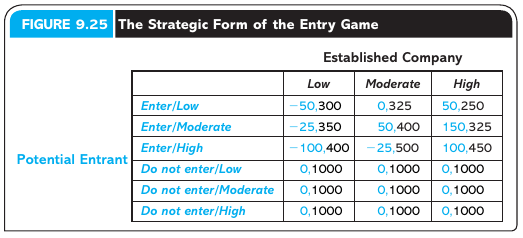
\includegraphics[width=.9\textwidth]{figures/fig925.png}
  \end{center} 
  Can you find NE which are \textit{not subgame-perfect}?
\end{frame}

% - - - - - - - - - - - - - - - - - - - - - - - - - - - - - - - - - - - - - - - 

\begin{frame}{Deterrence of Entry}
  Consider \{Do not enter/Moderate, Low\}:
  \begin{itemize}
    \item Given no entry, established company always gets 1,000
    \item So planning to set a low price in post-entry game is optimal for est. company
    \item Given that est. company prices low, new company has no regrets staying out 
    \item If new company enters when est. company sets low price, the best they can do is \textit{moderate} and earn -25
  \end{itemize}
\end{frame}

% - - - - - - - - - - - - - - - - - - - - - - - - - - - - - - - - - - - - - - - 

\begin{frame}{Deterrence of Entry}
  Consider \{Do not enter/Moderate, Low\}:
  \begin{itemize}
    \item Why is this \textit{not} subgame-perfect?
    \item Consider what happens if the new company doesn't believe the threat, 
    and actually \textit{does} enter
    \item Then the established firm would actually be better off by setting a \textit{moderate} price
    \item So we say that the threat of low price competition was not a \textbf{credible} threat
  \end{itemize}
\end{frame}

\begin{frame}{Deterrence of Entry}
  So what should the CEO of an established company do? 
  \begin{itemize}
    \item How can they commit to an aggressive pricing strategy that they know they won't follow through on? 
    \item What if there is a \textit{costly} investment in a new technology which has an investment cost of 500,
    but lowers per-unit production costs
  \end{itemize}
\end{frame}

\begin{frame}{Deterrence of Entry}
  \begin{center}
    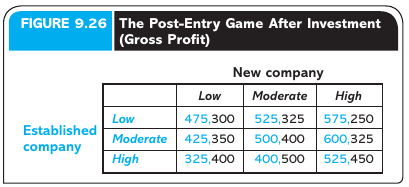
\includegraphics[width=.8\textwidth]{figures/fig926.png}
  \end{center} 
  What is the NE of this new post-entry game?
\end{frame}

\begin{frame}{Deterrence of Entry}
  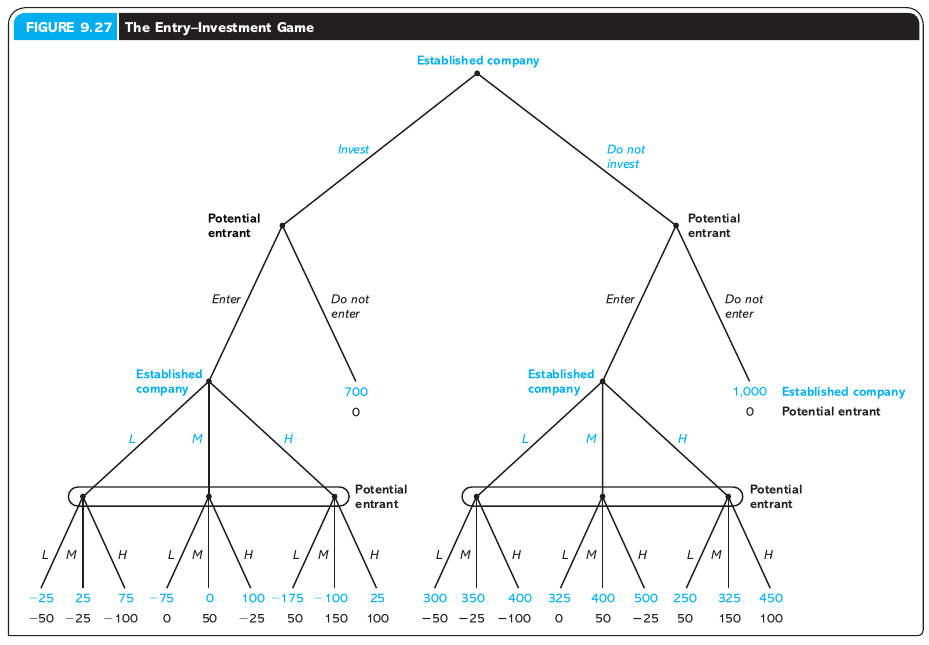
\includegraphics[width=1\textwidth]{figures/fig927.png} 
\end{frame}

\begin{frame}{Deterrence of Entry}
  \begin{center}
  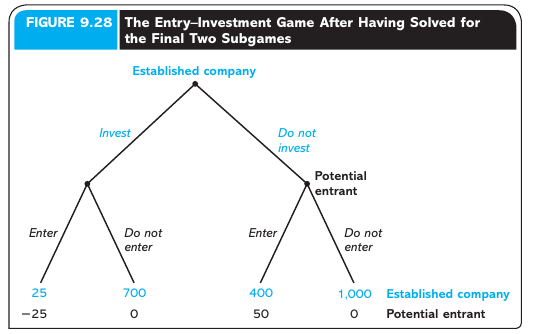
\includegraphics[width=.8\textwidth]{figures/fig928.png}
  \end{center}
  What is the \textbf{SPNE} now?
  \begin{itemize}
    \item Is the aggressive pricing strategy \textit{credible} now? 
  \end{itemize}
\end{frame}

\begin{frame}{Deterrence of Entry}
  \begin{center}
    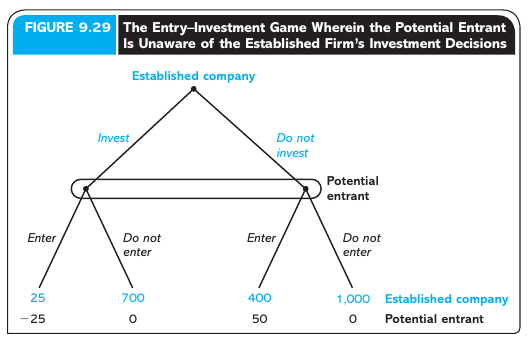
\includegraphics[width=.7\textwidth]{figures/fig929.png} 
  \end{center}
  Consider the importance of communicating the investment
  \begin{itemize}
    \item What is the SPNE when the potential entrant can't see whether the established company has invested? 
  \end{itemize}
\end{frame}

\begin{frame}{A Doomsday Device}
  Spoilers for \textit{Doctor Strangelove or: How I Learned to Stop Worrying and Love the Bomb} (1964)
  \begin{quote}
    \footnotesize
    \textbf{Dr. Strangelove:} Mr. President, it is not only possible, it is essential. That is the whole idea of this machine, you know. Deterrence is the art of producing in the mind of the enemy . . . the fear to attack. And so, because of the automated and irrevocable decision making process which rules out human meddling, the doomsday machine is terrifying. It’s simple to understand. And completely credible, and convincing. (Turning to DeSadeski.) But the whole point of the doomsday machine is lost if you keep it a secret! Why didn’t you tell the world, eh?

    \textbf{Soviet Ambassador DeSadeski:} It was to be announced at the Party Congress on Monday. As you know, the Premier loves surprises.
  \end{quote}
\end{frame}



\end{document}
